\chapter{Introdução ao BI}\label{cap_trabalho_academico}

% https://www.researchgate.net/publication/273861123_Why_Business_Intelligence_Significance_of_Business_Intelligence_Tools_and_Integrating_BI_Governance_with_Corporate_Governance

De forma geral, o termo \textit{Business Intelligence} (BI) ainda não é bem definido na literatura, mas alguns dos principais estudiosos da área, como Solomon Negash, apresentam o BI como um sistema que combina dados operacionais com ferramentas analíticas para apresentar informações para os gerentes do negócio. O objetivo disso é melhorar a qualidade das decisões do processo, tornando-as melhor embasadas, então os métodos do BI podem ser usados para melhor entender o estado da empresa, organização ou órgão onde estiver sendo aplicado, resultando em melhores decisões \cite{negash1}. Apesar disso, ainda existe bastante empresa que emprega o BI num viés muito mais ligado à gestão, sem exigir muito conhecimento da parte de tecnologia da informação, e usando conceitos sobre mercado, marketing, administração da produção etc.

Nesse trabalho serão usados os conceitos que se aproximam mais ao que Negash apresenta como BI, e dentro do que ele define como sendo importante na Inteligência de Negócios podemos citar algumas áreas do conhecimento como:

\begin{itemize}
	\item \textit{Data Warehouse}
	\item Visualização
	\item Mineração de dados
	\item \textit{Online Analytic Processing} (OLAP)
	\item Gerenciamento do conhecimento
	\item Probabilidade
	\item Estatística
	\item Análises preditivas
	\item Detecção de anomalias
\end{itemize}

\section{Estrutura básica do BI}

Como foi apresentado anteriormente, o BI serve para auxiliar nas tomadas de decisão, e isso é alcançado usando os dados da empresa ou órgão em que estiver sendo empregado. Os dados são armazenados em \textit{Data Warehouses}, que são armazéns de dados, em tradução livre, esses armazéns guardam dados históricos, então a partir deles é possível analisar o desenvolvimento de variáveis importantes e o comportamento delas de acordo ao passar dos anos e tentar estabelecer padrões, isso por si só já poderia ser usado para prever possíveis mudanças em estratégia de negócios \cite{negash1}.

Após o armazém, os dados devem ser coletados e limpos, a limpeza corresponde a remoção de linhas erradas, que contenham dados ou errados ou faltosos, que podem atrapalhar na análise e apresentação ao gestor. Em seguida, os dados são apresentados à pessoa do negócio, que a partir das suas análises irá tomar alguma decisão que afeta a estratégia da empresa. Com alguma sorte essa decisão será pautada em matemática, estatística e informações úteis, sendo bem embasada em dados e números.

De forma resumida, o BI usa o Data Warehouse para guardar os dados, usa um conjunto de ferramentas e técnicas para limpar e extrair os dados, essa técnica também é conhecida como \textit{Extraction, Transform, Load} (ETL), e ,finalmente, apresenta gráficos que mostram o comportamento de variáveis de interesse da empresa para o gestor, que a partir disso escolhe alguma estratégia para os rumos da empresa/órgão/setor que gerencia.

\begin{figure}[h]
	\centering
	
\includegraphics[scale=0.80]{./figures/cap1/resumo_bi.png}
	\caption{Resumo de um sistema BI}
\end{figure}

Isso tudo que foi tratado acima corresponde às etapas do processamento de dados estruturados, ou seja, dados que podem ser organizados e categorizados em linhas e colunas, e que, muitas vezes, possuem relações entre si. O processo para "manusear" dados não estruturados é um pouco diferente porque eles não são tão bem organizados, e alguns passos precisam ser inseridos nesse caminho para que eles sejam apresentados e tratados da melhor forma, evitando distorções.

\section{Visualização de dados no BI}

Todas as etapas do processo são importantes, mas o gestor só enxerga o último estágio: a visualização, e as decisões serão tomadas a partir das conclusões tiradas da visualização, portanto, a visualização precisa de um cuidado especial, o visual é importante porque ele pode levar a conclusões erradas, então é necessário ter atenção com as cores, os eixos entre outros detalhes \cite{claus1}.

No painel feito as tabelas são bastante usadas, elas são uma importante ferramenta para visualização de dados, mesmo assim, a aparente simplicidade pode fazer com que não recebam a atenção devida. 
\section{Ferramentas de BI}

Existem vários programas feitos para se desenvolver painéis BI, entre os mais usados podemos citar o PowerBI, Pentaho, Tableau entre outros. Na JFRN o software usado é o Qlikview. 

Ultimamente as empresas que fornecem os softwares de BI têm notado que uma abordagem de serviços é mais rentável, então o cliente paga por um serviço e não por um produto. As mensalidades variam de acordo com o serviço que o cliente quiser, ficando mais caro à medida que mais funções são adicionadas ao pacote que será usado. Abaixo serão listados alguns dos principais serviços de BI do mercado.

\subsection{Power BI}

O Power BI é um serviço da Microsoft, ele tem por objetivo fornecer visualização de dados, customizável pelo próprio usuário, e também funções de BI que sejam simples de serem feitas. 

Em 2020 o preço dos serviços partem de \$9,99 para o Power BI Pro e \$4,995 para o Power BI Premium, é importante ressaltar que em ambos os casos esses valores são mensais, e o pacote que atende às necessidades da JFRN é o mais caro, que pode aumentar o preço de acordo com as funcionalidades extra que serão requeridas para atender às demandas.

\begin{figure}[h]
	\centering
	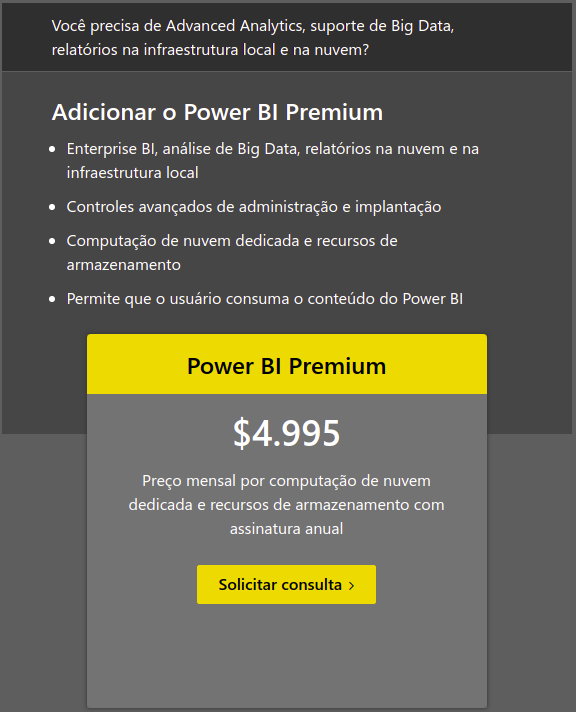
\includegraphics[scale=0.40]{./figures/cap1/powerbi.png}
	\caption{Preço do Power BI Premium}
\end{figure}

\subsection{Qlikview}

O Qlikview é um software desenvolvido pela Qlik, que tem focado os esforços no desenvolvimento do Qlik Sense, que começou como um produto paralelo e agora é o principal. Então, o suporte ao Qlikview está entrando no fim e nem é mais possível consultar os preços dele no site da Qlik. 

Apesar disso, o Qlikview é uma boa ferramenta, oferece um bom conjunto de funções para analisar e apresentar os dados. O Qlik Sense é a evolução dele, com muito mais recursos.

%https://primaconsulting.co.uk/news/2018/3/26/qlikview-vs-qliksense
\subsection{Tableau}

Tableau é uma solução que fornece funcionalidades clique-e-arraste para ajustar dados, criar painéis e visualizações. Existem três produtos dentro dele, o Tableau Desktop, Server e o Online. O preço entre eles varia de \$12,00 até \$70,00 por mês, por licença, podendo ajustar anualmente. É uma das ferramentas mais simples e completas do mercado, exigindo pouco conhecimento do analista por ser clique-e-arraste, por outro lado isso torna um pouco mais difícil o desenvolvimento de análises mais detalhadas.

De modo geral, as principais ferramentas disponíveis são muito similares entre si, todas são competentes, fornecem ótimas funcionalidades, possuem um bom suporte e custam um valor razoavelmente alto, principalmente com o câmbio desfavorecendo o Real. Porém, as ferramentas proprietárias não são as únicas, e para o desenvolvimento do Painel do Centro de Inteligência o Python foi escolhido.



%https://www.betterbuys.com/bi/tableau-pricing/


